% !TEX root = dissertation2.tex
\chapter{Results}

% Purpose
\section{Purpose}
The researcher sought to determine the viability of RTK GNSS augmentation to asses railway infrastructure and act as a reliable track vehicle locator capable of meeting the requirements of a location determination system as defined by the FRA by answering these questions:

1)\emph{Hump Yard Profile:}
Can a locomotive use RTK augmented GPS to measure the  vertical profile of bowl tracks in an automatic classification yard during production activities?

2)\emph{Horizontal Track Alinement:}
Can a common track vehicle use RTK augmented GPS/GNSS to determine the horizontal degree of curvature ($D_c$) comparable with specialized track geometry vehicles?

3)\emph{Track Occupancy:}
Can a common track vehicle use RTK augmented GPS/GNSS to meet the positioning requirements for track occupancy outlined by the FRA~\citep[pp.6-7]{1995FRADiffe} for a location determination system?

These experiments used common track vehicles equipped with survey-grade RTK GPS/GNSS instrumentation across yard and mainline track. The research examined three absolute positioning applications using RTK augmented GPS/GNSS in the context of a Class I railroad. The experiments addressed these questions:

1. \emph{Hump Yard Profile}\\
%Relative precision - Precision is defined as a measure of the tendency of a set of numbers to cluster about a number determined by the set (e.g. the mean). The usual measure is the standard deviation with respect to the mean. Relative precision denotes the tendency for the various components (X, Y, Z) between one station and other stations in the network to be clustered about the adjusted values. Current custom is to express relative precision at the two-standard deviation (95% confidence) level. This may be stated in terms of a relative error ellipse or as a proportion of the separation distance (e.g. 10 ppm or 1:100,000). 
Can a locomotive equipped with RTK GPS instrumentation be used to measure the  vertical profile of bowl tracks in an automatic classification yard during humping operations?
The question was answered through the completion of several objectives:
\begin{itemize}
\item A method was developed for measuring track profiles in the bowl area of an active hump yard.
\item The method was demonstrated by use of an ad hoc GPS reference station transmitting correctors to a RTK GPS receiver aboard a yard locomotive. 
\item A relative vertical precision distribution was determined from the RTK GPS observations.
\item Track profiles were developed from the locomotive survey data.
\end{itemize}

2. \emph{Horizontal Track Alinement}\\
Can a common track vehicle use RTK augmented GPS/GNSS observations to determine the horizontal degree of curvature over tangent track comparable with specialized track geometry vehicles?
The question was answered through the completion of several objectives:
\begin{itemize}
\item A method was developed for measuring track horizontal position from a track inspector's Hi-Rail vehicle.
\item A software model was developed to determine the degree of curvature using the string lining method.
\item A parameter estimation of the ${D_c}$ variability of the model and a track geometry car was determined for selected tangent track segments.
\end{itemize}

3. \emph{Track Occupancy}\\
Can a common track vehicle using RTK augmented GPS/GNSS instrumentation meet the positioning requirements for track occupancy outlined by the FRA for a location determination system?
The question was answered through the completion of several objectives:
\begin{itemize}
\item An analytical method was developed to determine the variance in a series of RTK GNSS measured track positions from specific geometric segments.
\item A hypothesis test was used to determine the likelihood of RTK GNSS position measurements to meet the FRA criteria for reliable track occupancy.
\end{itemize}

\section{Hump Yard Profile Results}
The objective of experiment one was to use a locomotive to survey an active hump yard to produce track profiles from RTK augmented track observations. A hump yard owned by CSXT and located in Hamlet North Carolina was the subject of this experiment. Track centerline top-of-rail observations recorded from locomotive and ground observations are summarized in \ref{tab:humpData}. The human effort expended during the yard survey is presented in table \ref{tab:labor}.
% Table of human resource usage
\begin{center}
\begin{table}[!ht]
\caption{Hump Yard Survey Human Resource Utilization}\label{tab:labor}
\begin{tabular}{llll}%{ p{4cm} p{3cm} p{4cm}}
\toprule
Classification & Labor Hours & Task Description\\
\midrule
Surveyor, locomotive & 5 shifts of 8 hours & manage locomotive GPS  & \\
Locomotive operator & 5 shifts of 8 hours & manage locomotive, switches & \\
Surveyor, ground & 2 sessions of 3 hours & collect POI, set bench marks & \\
Watchmen lookout & 2 sessions of 3 hours & safety lookout for ground surveyor\\
Company escort & 5 hours & safety briefings, guide\\
\bottomrule
Total hours & 97 hours &\\
\end{tabular}
\end{table}
\end{center}
%An analysis of the vertical precision of the observations will be used to determine if statistical evidence is present to indicate the one sigma mean vertical precision of RTK augmented GPS observations by locomotive in a hump yard is 0.1 feet or less.
The resulting OPUS reports generated from the two reference station observation sessions referred to in chapter 3, page \pageref{baseRefPeriod} are exhibited in Appendix A, pages \pageref{opus1}~-~\pageref{opus2}.

Adjustments to the autonomous GPS position of the ad hoc reference station (CP1) used during the survey are listed in table \ref{tab:AdHocPos}. An error of 0.003 feet was introduced in the elevation adjustment of CP1. The likely cause was in transcribing the calculated elevation adjustment into the TGO software. Consequently, the transcription error was propagated to each observation during recomputing point positions from the base station to observation vectors. The error was not significant to the work, as it was less that half the manufacturer's stated $\pm$~0.066 foot vertical accuracy of the GPS total station.

 % Table of reference station corrections
\vspace{-30pts}
\begin{center}
\begin{threeparttable}
	\caption{Reference Station Adjustment}
	\label{tab:AdHocPos}
	\begin{tabular}{l c c c}
	\toprule
	Point & Northing & Easting & Elevation\\
	\midrule
	CP1 autonomous & 426094.534 & 1802674.100 & 462.354 \\
	OPUS 89691472 & 426095.398 & 1802677.668 & 464.944  \\
	OPUS 89691491 & 426095.376 & 1802677.685 & 465.107  \\
	mean OPUS & 426095.387 & 1802677.677 & 465.026 \\
	\midrule
	EB1559 publlished& 422425.72 & 1795001.00 & 389.54 \\
	CP1 to EB1559 vector & $\Delta$-3721.022 & $\Delta$-7653.073 & $\Delta$-77.070 \\
	\midrule
	CP1 adjusted & 426095.387 & 1802677.677 & 465.081\tnote{} \\
	\midrule
	residuals&&&\\
	$\Delta$ OPUS & 0.000 & 0.000 & +0.055\\
	$\Delta$ EB1559 & +0.068 & -0.045 & +0.003\\
	\bottomrule
	\end{tabular}
%	\begin{tablenotes}
%		\item[\dag]{Elevation adjusted to EB1559.}
%	\end{tablenotes}
\end{threeparttable}
	\end{center}

Two TEQC reports were generated from the two reference station observing sessions. The reports detail the quality of observations by the reference station during the periods referenced in chapter three page \pageref{baseRefPeriod} referenced in Appendix A, pages \pageref{teqc1} and \pageref{teqc2}. The overview graphically depicts the GPS SVs visible during the base station observation period. Additional information in the reports the quality of reference station observations.

% Table of Hump Yard Results
\begin{table}[ht]
	\begin{center}
	\caption{Relative Vertical Precision Summary}
	\label{tab:humpData}
	\begin{tabular}{c c c c c c}
	\toprule
	$\alpha$ = 0.01&&&conf.int.&&conf.int.\\
	Tracks & N & $\mu$ &$\mu$& $\sigma$&$\sigma$\\
	\midrule
	58 & 9,570 & 0.07753 & 0.07640 to 0.07866 & 0.0429 & 0.04213 to 0.04373\\
	\bottomrule
	\end{tabular}
	\end{center}
\end{table}

% Shot list

% Spreadsheets
Spreadsheets were constructed in Google Docs, and shared among the research team. A workbook was created for each track group, and individual worksheets constructed for each track. Algorithms for determining horizontal linear reference and elevation scaling are available. A hyperlink to each group workbook is exhibited in Appendix A, page .

% Profile drawings
Track profiles were plotted with a drawing provided by CSX as the result of a January 2001 survey by others. Attempts at recovering the 2001 benchmarks were unsuccessful.

The horizontal axis of each drawing represented the horizontal linear track reference and the vertical axis representing the elevation. A reference mark on the drawing was matched with the track structure observed during the survey. Linear references from the drawing were assigned to the match mark in the spreadsheet, and the linear reference of each track observation was determined by horizontal stationing equation \ref{eq:horzSta} . 

Elevations were plotted twice, first in a 1:1 scale with the design yard grade, and secondly exaggerated 5:1 to better discern profile differences. Entries in table \ref{tab:profiles} Appendix A, page \pageref{profiles} are hyperlinks to D size drawings (.pdf format). 

% Relative vertical precision
The relative vertical precision of each point observed calculated by mobile\#1 was recorded. The descriptive statistics for the relative vertical precision is listed in table \ref{tab:humpData}.

Appendix A figure \ref{vert_hist} presents a histogram of the vertical precisions in addition to descriptive statistics for the aggregate observations.

\emph{Hump Yard Profile Summary}

An RTK survey of the Hamlet Terminal by locomotive was completed in five, eight hour shifts. The first day was consumed by yard safety, yard facility familiarization, and antenna alignment. Four eight hour shifts were sufficient to complete a traverse of every open track in the bowl. The survey strategy first traversed the pullout end to the foul point. The pull-out end humpmaster preplanned and coordinated runs through alley\footnote{A clear track.} track with the locomotive engineer, though the survey locomotive was also sporadically used to pull cars during the survey.

The hump end was surveyed during the last day's shift change. During shift change, the pin puller and other hump end personnel undergo a transition period of exchanging relevant yard information, with the oncoming shift receiving a current safety briefing. The hump-end yard master took advantage of the staggered shift change to switch the survey locomotive through each hump and group lead track on the hump end. The brief period between shift changes did not allow time for individual group lead and tracks to be renamed in the survey controller. Consequently the data was separated manually during post-survey office work.

Post survey work consisted of adjustment to the reference station position; recalculating point positions from station to point vectors; deconstructing the aggregated points by track and lead; separating points into layers based on track and lead; adjusting ground points so as to be coincident with the centerline; renaming point sequences and exporting each sequence to a spreadsheet; applying a linear reference to each point; scaling the elevations in preparation to plot on an existing CAD drawing; plotting and printing the CAD generated profiles.

\section{Determining Alinement by Hi-Rail Results}
%Experiment 2 Analysis

Mainline track was surveyed by table \ref{tab:instruments} mobile\#2, mounted to a track inspector's Hi-Rail, over mainline track listed in table \ref{tab:Hi-RailSurvey}.

Continuous data recording during the 20 January 2010 survey was impeded by unexpected receiver operation. The receiver was unable to initialize with a new VRS without cycling receiver power after each VRS update. The problem lead to numerous unexpected data gaps during the traverse. The problem was identified and corrected by updating the receiver firmware. The receiver performed as expected during subsequent surveys. Mainline surveys traversing the Kanawaha Subdivision from mile post (MP) 494 to 523 are summarized in table \ref{tab:Hi-RailSurvey}.

% Mainline Survey Inventory
\begin{table}[ht!]
	\begin{center}
	\caption{RTK Surveys By Hi-Rail}
	\label{tab:Hi-RailSurvey}
		\begin{tabular}{c c c c c l}
			\toprule
			Ref.&Date& Traverse&Track(s)&CL Observations&Note\\
			\midrule
	A & 20 January 2010   &MP494 to 523 & 1,2           & 18,095 &f/w 1.02\\
	B & 5 February 2010   &MP495 to 512 & 2,1,2        & 15,225 &f/w1.13, traffic \\
	C & 14 February 2010 &MP495 to 523 & 1, 2          & 22,866 &f/w1.13\\
	D & 3 March 2010       &MP495 to 522 & 2,3,2        & 19,993 &f/w1.13\\
	E & 18March 2010      &MP494 to 523  & 1             & 21,001 &f/w1.13\\
			\bottomrule
	\end{tabular}
	\end{center}
\end{table}

Output generated from processing RTK observations with string line model are cataloged in Appendix B. The rail company provided track chart precedes each segment between MP494 and 523 traversed by a RTK equipped HI-Rail. Correlation between model output and charted features is produced in table \ref{tab:Hi-RailTraverse}. 

Two discrepancies between the track chart values and model output were discovered.
\begin{itemize}

\item The track charts indicates the curve beginning at MP {508.9} is a curve to the right (referenced to the direction of travel, increasing mile post). The model determined the a curve was to the left. The model determined value is verified by examination of a plan view of the track observations between MP 508 and 509, figure \ref{crv508_9}.
\begin{figure}[!ht]
	\begin{center}
	\vspace{0pt}
	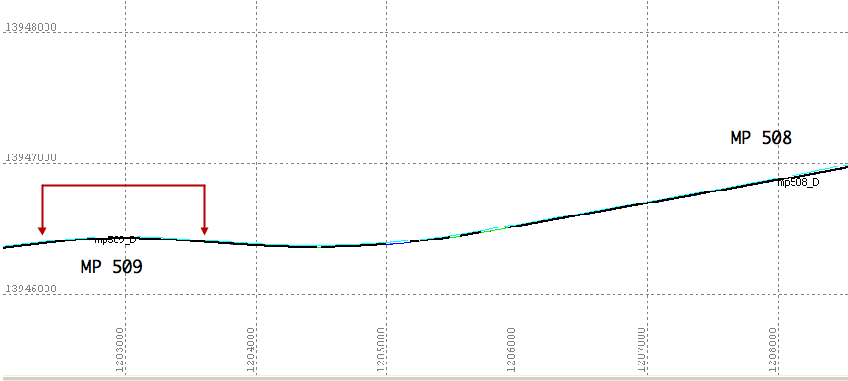
\includegraphics[scale=0.30]{graphics/508_9curve}
	\caption{Plan View MP 508-509}
	\label{crv508_9}
	\end{center}
	\vspace{-10pt}
\end{figure}

\item The track chart indicates the 1 degree curve to the right at mile post 521.15 extends approximately 0.15 miles. The model determined the curve extends from MP 521.15 to 521.83, or one half mile longer than indicated on the track chart. The model determined value is verified by examination of a plan view of the track observations between MP 521 and 522, as illustrated by figure \ref{crv521}.

\begin{figure}[!ht]
	\begin{center}
	\vspace{0pt}
	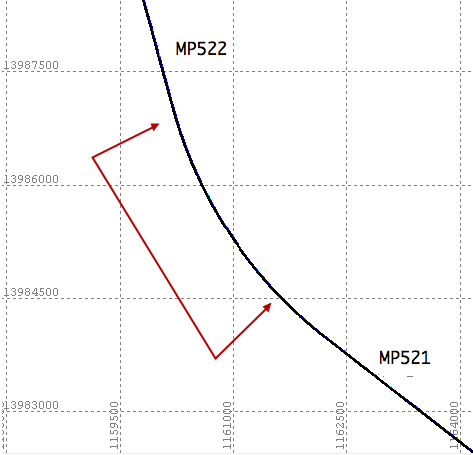
\includegraphics[scale=0.30]{graphics/521-522curve}
	\caption{Plan View MP 521-522}
	\label{crv521}
	\end{center}
	\vspace{-10pt}
\end{figure}

\end{itemize}

Features causing loss of GNSS signal (LOS) were documented by referencing the location to the track chart. When not evident from the track chart, the geodetic coordinates of a point before LOS was entered into Google Maps, and the aerial image examined. This method was effective in determining the location of signal bridges and several overpasses.

Table \ref{tab:Hi-RailTraverse} also references rail company track chart (TC) values for ${D_c}$ and mile length for comparison with the model output. Track charts do not provide exact values for individual tracks, therefore the comparison serves only to verify the quantity and magnitude of alinement features.

\begin{center}
% Setup for longtable
\begin{longtable}{c l c l}
\caption[RTK Hi-Rail Traverse MP 494-523, Alinement Annotation]{RTK Hi-Rail Traverse MP 494-523, Alinement Annotation}
\label{tab:Hi-RailTraverse} \\
%This is the header for the first page of the table...
\hline
   \multicolumn{1}{c}{\textbf{MP Reference}} &
   \multicolumn{1}{l}{\textbf{Feature}} &
   \multicolumn{1}{c}{\textbf{TC Value}} &
   \multicolumn{1}{l}{\textbf{Note}} \\
\hline
\endfirsthead

%This is the header for the remaining page(s) of the table...
\multicolumn{4}{c}{{\tablename} \thetable{} -- Continued} \\[0.5ex]
\hline
   \multicolumn{1}{c}{\textbf{MP Reference}} &
   \multicolumn{1}{l}{\textbf{Feature}} &
   \multicolumn{1}{c}{\textbf{TC Value}} &
   \multicolumn{1}{l}{\textbf{Note}} \\
\hline
%  \\[-1.8ex]
\endhead

%This is the footer for all pages except the last page of the table...
\midrule
\multicolumn{4}{r}{{Continued next page\ldots}} \\
\endfoot

%This is the footer for the last page of the table...
\bottomrule
\endlastfoot
494-495 & mile length & 8,858' &  Hi-Rail:8,949' \\
	494.05&curve&$3^{\circ}$03'R&\\
	494.46&curve&$2^{\circ}$45'L&\\
	494.65&curve&$2^{\circ}$30'R&\\
495-496 & mile length & 5,295' &  Hi-Rail:5,414' \\
	495.05&curve&$2^{\circ}$30'R&\\
	495.46&curve&$2^{\circ}$30'L&\\
	495.6-495.7&I-64 overpass&&LOS\\
\hline
496-497 & mile length & 5,255' &  Hi-Rail: 5,323' \\	
	496.05&curve&$3^{\circ}$45'L&\\
	496.25&curve&$1^{\circ}$00'L&\\
497-498 & mile length & 5,276' &  Hi-Rail: 5,340' \\
	497.3&curve&$0^{\circ}$45'L&\\
	497.61& & & LOS, VRS update\\
498-499 & mile length & 5,290' &  Hi-Rail: 5,342' \\
	498.6&curve&$2^{\circ}$00'R&\\
499-500 & mile length & 5,283' &  Hi-Rail: 5,342' \\
500-501 & mile length & 5,280' &  Hi-Rail: 5,356' \\
	500.4&curve&$2^{\circ}$32'R&\\
\hline
	501.03-501.12&cross over&&cross over, track 1 to 1\\
	501.15-501.35&Guyandotte River Bridge&&LOS\\
	501.35&curve&$4^{\circ}$14'L&\\
	501.6-501.67&29th Street overpass&&LOS\\
	501.9&curve&$1^{\circ}$33'L&\\
	501.95&curve&$1^{\circ}$33'R&\\
501-502 & mile length & 5,266' &  Hi-Rail: 5,316' \\
	502.62-502.69&cross over&&track 2 to 1\\
502-503 & mile length & 5,383' &  Hi-Rail: 5,208' \\
	503.4&curve&$1^{\circ}$15'L&\\
	503.55&curve&$1^{\circ}$33'R&\\
504-505 & mile length & 5,196' &  Hi-Rail: 5,281' \\
	504.05&curve&$2^{\circ}$56'R&\\
	504.15&curve&$4^{\circ}$30'L&\\
	504.52&curve&$0^{\circ}$55'R&\\
	504.6&curve&$1^{\circ}$05'L&\\
	504.85&curve&$2^{\circ}$00'L&\\
	504.92-504.96&signal bridge&&LOS\\
505-506 & mile length & 5,286' &  Hi-Rail: 5,335' \\
	505.0&spiral&from $2^{\circ}$00'L&\\
	505.5&curve&$1^{\circ}$00'R&LOS@505.55\\
\hline
506-507 & mile length & 5,189' &  Hi-Rail: 5,256' \\
	506.24&curve&$0^{\circ}$32'L&\\
	506.34-506.41&17th Street interchange&&LOS\\
	506.7-507.78&signal bridge&&LOS\\
	506.78&curve&$1^{\circ}$55'R&\\
507-508 & mile length & 5,255' &  Hi-Rail: 5,327' \\
	507.95&curve&$0^{\circ}$23'R&\\
508-509 & mile length & 5,262' &  Hi-Rail: 5,337' \\
	508.37-508.57&Spring Valley Road overpass&&LOS\\
	508.57&curve&$0^{\circ}$45'R&\\
	508.65&signal bridge&& LOS \\
	508.9&curve&$1^{\circ}$18'R&TC error, left\\
509-510 & mile length & 5,280' &  Hi-Rail: 5,355' \\
	509.0&spiral&$1^{\circ}$18'R  & TC in error, left\\
	509.21&curve&$0^{\circ}$18'L&\\
	509.56&curve&$0^{\circ}$28'L&\\
510-511 & mile length & 5,280' &  Hi-Rail: 5,336' \\
	510.2&curve&$1^{\circ}$05'R&\\
	510.7&curve&$3^{\circ}$23'R&\\
	510.95&signal bridge& &LOS\\
\hline
511-512 & mile length & 5,231' &  Hi-Rail: 5,319' \\
	511.72-511.8&Norfolk Southern overpass&&LOS\\
512-513 & mile length & 5,249' &  Hi-Rail: 5,349' \\
	512.52-513&Big Sandy River Bridge&&LOS\\
513-514 & mile length & 5,264' &  Hi-Rail: 5,408' \\
	513.0&curve&$4^{\circ}$51'R&\\
	513.31&signal bridge& &multipath\\
	513.6&curve&$6^{\circ}$23'L&\\
	513.7&curve&$3^{\circ}$00'R&\\
	513.92&curve&$3^{\circ}$00'L&\\
514-515 & mile length & 5,263' &  Hi-Rail: 5,293' \\
	514.0   &curve&$3^{\circ}$00'L& \\
	514.2   &curve&$2^{\circ}$00'R& \\
	514.8   &curve&$2^{\circ}$00'L& \\
	514.55 &signal bridge& &LOS\\
515-516 & mile length & 5,240' &  Hi-Rail: 5,318' \\
	515.0 &curve&$0^{\circ}$45'L& \\
	515.2 &curve&$1^{\circ}$30'R& \\ 
	515.5 &curve&$1^{\circ}$15'R& \\
	515.6 &signal bridge& &LOS\\
	515.8 &curve&$0^{\circ}$45'L& \\
\hline
516-517 & mile length & 5,047' &  Hi-Rail: 5,110' \\	
	516.12&curve&$3^{\circ}$00'R&\\
	516.78-517&curve&$1^{\circ}$00'L&LOS\\
517-518 & mile length & 5,432' &  Hi-Rail: 5,530' \\
	517.0&curve&$1^{\circ}$00'L & to $3^{\circ}$00'L\\
	517.43&curve&$1^{\circ}$30'L&\\
	517.6&curve&$4^{\circ}$15'L&\\
518-519 & mile length & 5,733' &  Hi-Rail: 5,821' \\
	518.05&curve&$1^{\circ}$00'R&\\
	518.23&curve&$1^{\circ}$15'L&\\
	518.4&curve&$0^{\circ}$00'&<sic>\\
	518.41&signal bridge& &multipath\\
	518.5&curve&$0^{\circ}$45'R&\\
519-520 & mile length & 4973' &  Hi-Rail: 5,059' \\
	519.1&curve&$1^{\circ}$30'L&\\
	519.15-519.34&2 signal bridges & &LOS\\
	519.2&curve&$1^{\circ}$00'R&\\
	519.6&curve&$2^{\circ}$00'L&\\
	519.65&curve&$2^{\circ}$00'R&\\
	519.8&curve&$2^{\circ}$30'L&\\
	519.9&curve&$1^{\circ}$45'R&\\
520-521 & mile length & 5,322' &  Hi-Rail: 5,431' \\
	520.5&curve&$2^{\circ}$15'R&\\
	520.55-520.69&Armco overpass& &LOS\\
\hline
521-522 & mile length & 4,972' &  Hi-Rail: 5,357.6' \\
	521.12-521.82&curve&$1^{\circ}$00'R&TC curve length error\\
522-523 & mile length & 5,023' &  Hi-Rail: 5,099' \\
	522.1-522.25&AK Steel Entrance Rd&&LOS\\
	522.6&curve&$1^{\circ}$00'L&\\
	522.9&curve&$0^{\circ}$30'L&\\
\end{longtable}
\end{center}
\vspace{-30pt}

% Measure method comparison between GMRS and Hi-Rail
To answer the research question asking if the RTK Hi-Rail method of determining $D_c$  was comparable with specialized inspection vehicles, measurements obtained from CSX for a GMRS inspection vehicle were compared with the output from the string line model using observations from a RTK GNSS equipped Hi-Rail. The two methods traversed CSX C\&O Ohio Subdivision between mile post 211 and 207. Illustration \ref{gmrs_HiRail} provides a graphic solution to the smoothed $D_c$ vs. mile post values obtained from both methods across the segment.

\begin{center}
\begin{longtable}{c c c c}
\caption[GMRS \& RTK Hi-Rail Comparision, MP 211-207, Alinement Annotation]{GMRS \& RTK Hi-Rail Comparision, MP 211-207, Alinement Annotation}
\label{tab:gmre_Hi-RailTrav} \\
%This is the header for the first page of the table...
\hline
   \multicolumn{1}{c}{\textbf{MP Reference}} &
   \multicolumn{1}{c}{\textbf{Feature}} &
   \multicolumn{1}{c}{\textbf{TC Value}} &
   \multicolumn{1}{c}{\textbf{Note}} \\
\hline
\endfirsthead

%This is the header for the remaining page(s) of the table...
\multicolumn{4}{c}{{\tablename} \thetable{} -- Continued} \\[0.5ex]
   \multicolumn{1}{c}{\textbf{MP Reference}} &
   \multicolumn{1}{c}{\textbf{Feature}} &
   \multicolumn{1}{c}{\textbf{TC Value}} &
   \multicolumn{1}{c}{\textbf{Note}} \\
\hline
%  \\[-1.8ex]
\endhead

%This is the footer for all pages except the last page of the table...
\midrule
\multicolumn{4}{r}{{Continued next page\ldots}} \\
\endfoot

%This is the footer for the last page of the table...
\bottomrule
\endlastfoot
	211-210 & mile length & 5,328' & GMRS:5,018' Hi-Rail:5,368' \\
	210.7     & curve &$2^{\circ}$15'L &\\
	210-209 & mile length & 5,263' & GMRS:4,973' Hi-Rail:5,314' \\
	209.6     & curve &$1^{\circ}$15'L &\\
	209.15   & curve &$1^{\circ}$00'L &\\
	209-208 & mile length & 5,252' & GMRS:5,027' Hi-Rail:5,318' \\
	208.8     & curve &$3^{\circ}$15'R &\\
	208.45   & curve &$1^{\circ}$15'L &\\ 
	208.0     & curve &$3^{\circ}$00'R &\\ 
	208-207 & mile length & 5,678' & GMRS:5,384' Hi-Rail:5,586' \\
	207.5     & curve &$5^{\circ}$00'R &\\ 
\end{longtable}
\end{center}

The longest tangent portion of the segment under study extends from MP 210.4 to 209.75, and was selected to determine the $D_c$ variance for the GMRS and the Hi-Rail RTK methods. An ideal measurement over an ideal tangent would result in an instantaneous $D_c$ value of zero at each point of measurement. The 201.4-209.75 tangent segment was assumed ideal. The variation from zero $D_c$ was determined for each method. Table \ref{tab:tanComp} provides descriptive statistics for $D_c$ values derived from each method. 

\begin{figure}[htpb]
	\begin{center}
	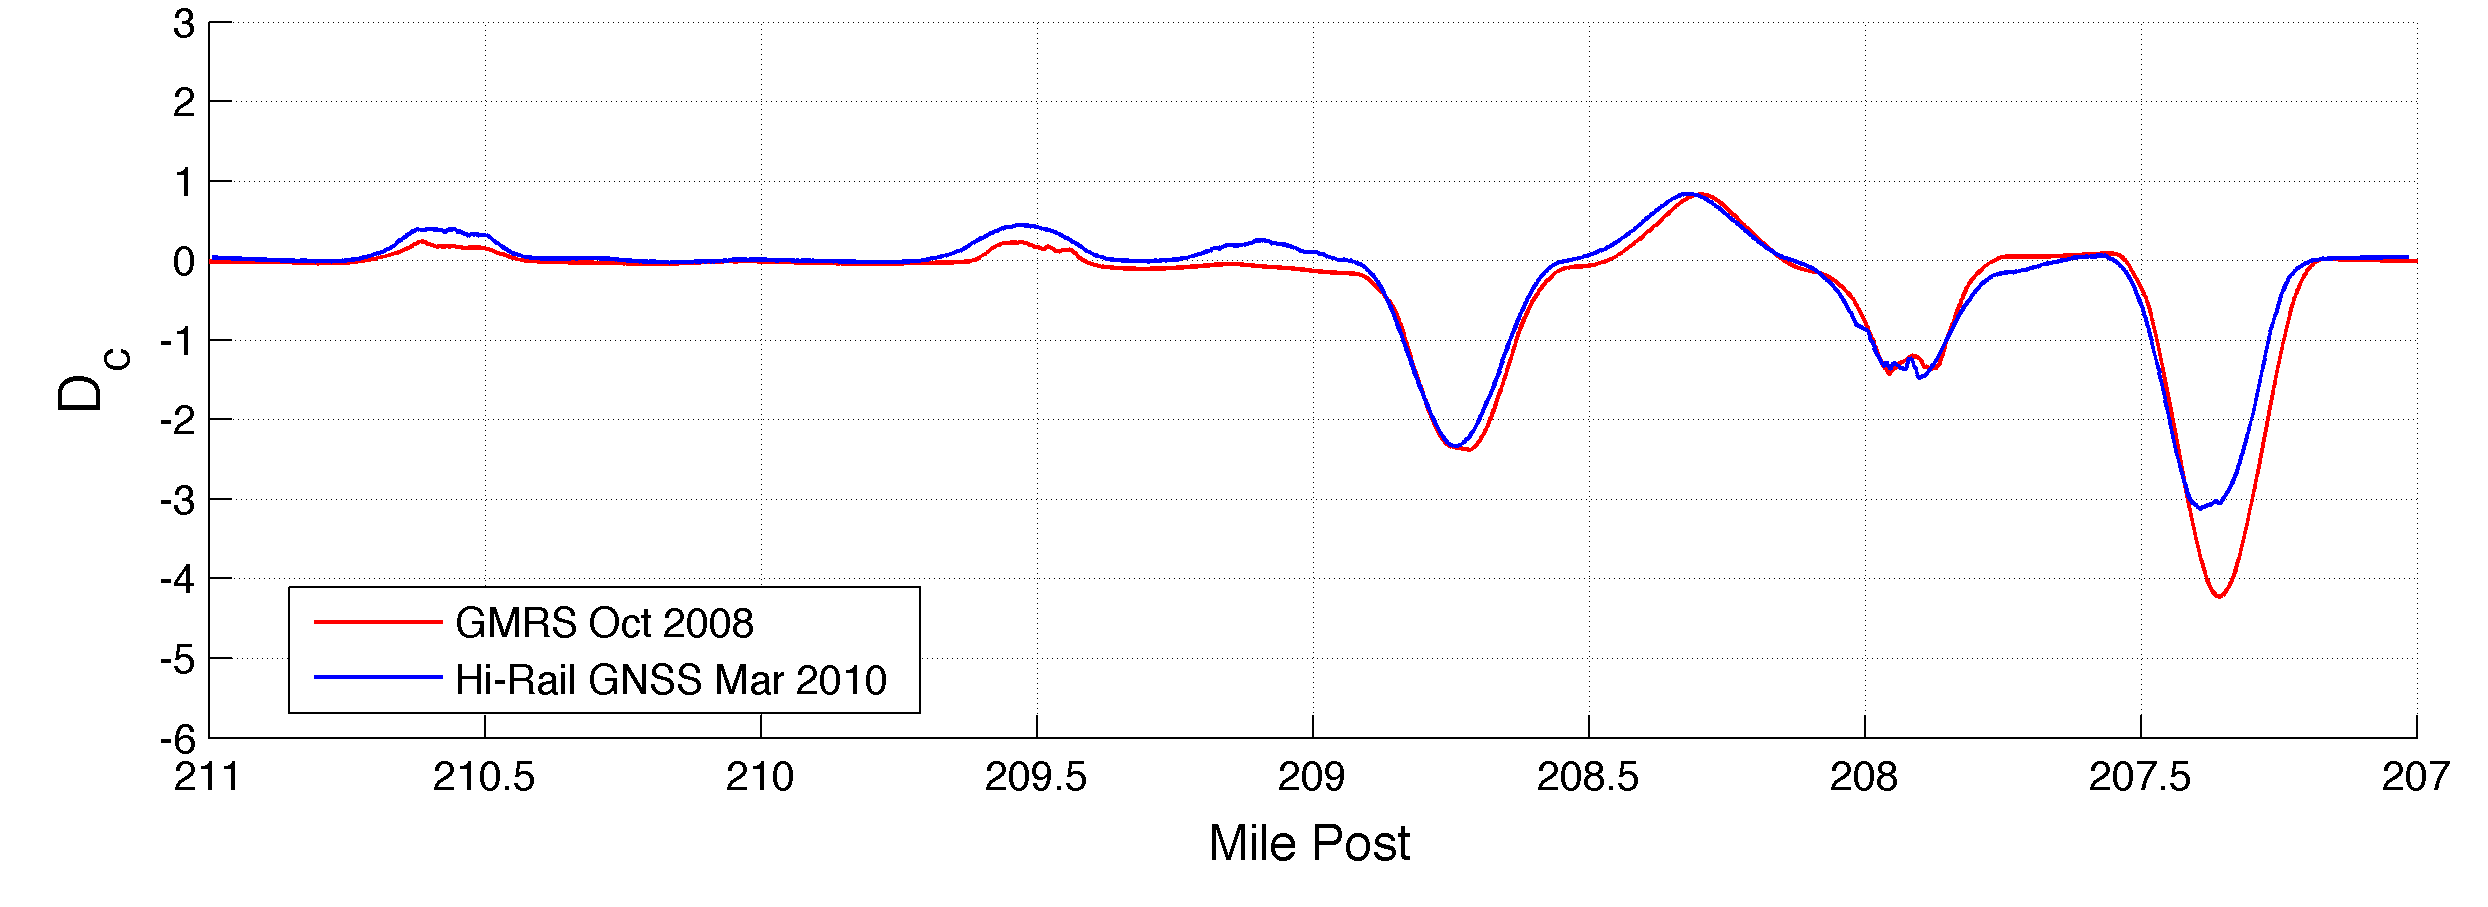
\includegraphics[scale=0.60]{graphics/GMRS_HiRail}
	\caption{GMRS and RTK GNSS Hi-Rail Comparison}
	\label{gmrs_Hi-Rail}
	\end{center}
\end{figure}

\begin{table}
\begin{center}
\caption{GMRS and RTK GNSS Hi-Rail Comparison, MP210.4-209.75 tangent}
\label{tab:tanComp}
\begin{tabular}{c c c c c c c}
\toprule
Vehicle&Stationing&N&${\mu}_{D_c}$&95\% CI&${\sigma}_{D_c}$&95\% CI\\
\midrule
GMRS&1 ft     &3,253&-0.02637&  -0.0307  -0.0219&0.1306&   0.1275   0.1339\\
Hi-Rail&15.5 ft&222   &-0.00417&-0.04106  0.03271&0.2789&0.2551   0.3076\\
\bottomrule
\end{tabular}
\end{center}
\end{table}

A histogram approximates the probability destiny function of the ${D_c}$ values. GMRS measurement deviation from zero is illustrated in figure \ref{gmrs_hist}. RTK GNSS Hi-Rail deviation illustrated in figure \ref{Hi-Rail_hist}. Both systems indicate a normal error distribution around zero ${D_c}$.

\begin{figure}[htpb]
	\begin{center}
	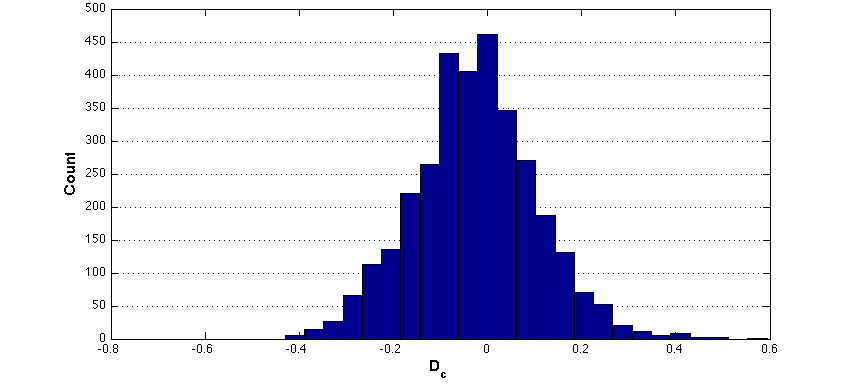
\includegraphics[scale=0.5]{graphics/GMRS_tanHist}
	\caption{GMRS ${D_c}$ Histogram, 210.4 to 209.75 tangent}
	\label{gmrs_hist}
	\end{center}
\end{figure}
\vspace{-40pt}
\begin{figure}[htpb]
	\begin{center}
	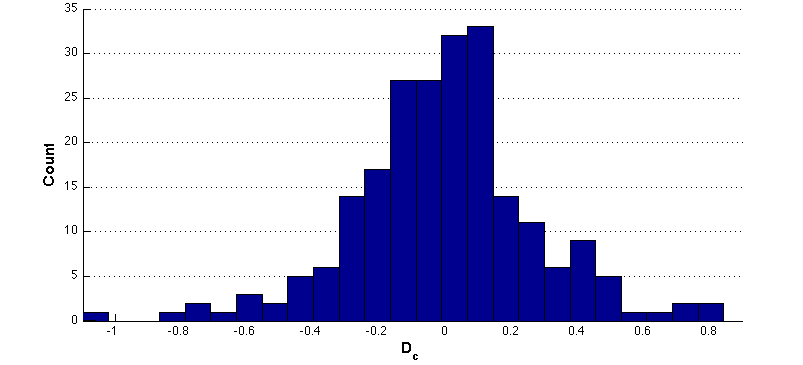
\includegraphics[scale=0.50]{graphics/HiRail_tanHist}
	\caption{Hi-Rail ${D_c}$ Histogram, 210.4 to 209.75 tangent}
	\label{Hi-Rail_hist}
	\end{center}
\end{figure}

%Track Occupancy Results
\section{Track Occupancy Results}
The question answered by experiment 3 was whether statistical evidence exists to determine if RTK GNSS as the sole position measurement instrument can meet the positioning requirements for track occupancy outlined by the FRA for a location determination system (LDS).

The question was answered through the completion of several objectives:
\begin{itemize}
\item An analytical method was developed to determine the variance in a series of RTK GNSS measured track positions from specific geometric segments surveyed by a common track vehicle.
\item A hypothesis test determined the likelihood of RTK GNSS position measurements in tangents and circular curves to meet the FRA criteria for reliable track occupancy.
\end{itemize}

The hypothesis test determines if sufficient statistical evidence exists to determine if RTK GNSS measurements conform to the criteria set by the FRA to enable the ability to distinguish what track a train in on in multi-track parallel segments.

Table \ref{tab:tanRegress} presents the result of a simple linear least squares regression performed on (Easting,Northing) coordinate pairs between mile post reference 498.9 and 500.2 for each of five surveys. Track position observations traversing three parallel tangent track of the same approximate length were recorded during five separate surveys. The correlation statistic ${R^2}$ for each regression was 0.99998 or better. The worse case variance around the centerline was exhibited on track 3. The regression excursive characterizes the observations of five surveys performed over a three month period for a section of tangent track over a mile in length.

\begin{table}[!htpb]
	\begin{center}
	\caption{Tangent Regression Coefficients, MP 498.9 to 500.2}
	\label{tab:tanRegress}
		\begin{tabular}{c c c c c c c}
\toprule
%\multicolumn{3}{l}{$\alpha = 0.00001$}\\
	Survey & Track & N  & Slope  & Y Intercept & Variance & Azimuth$^{\circ}$\\
\midrule
	A & 2 & 1,189 & 0.10220168 & 13825809.25 & 0.02259 & 264.164536\\
	B & 2 & 1,244 & 0.10219667 & 13825815.49 & 0.02208 & 264.164821\\
	C & 3 & 1,152 & 0.10208429 & 13825969.10 & 0.05664 & 264.171193\\
	D & 1 & 1,158 & 0.10213959 & 13825873.25 & 0.02432 & 264.168057\\
	E & 3 & 1,156 & 0.10209947 & 13825950.11 & 0.05338 & 264.170332\\
	\bottomrule
	\end{tabular}
	\end{center}
\end{table}

The cross-track error was determined between each point surveyed between mile post reference 498.9 and 500.2 and a centerline described from the regression coefficients of the tangent of survey A, presented in table \ref{tab:tanRegress}.
% Hypothesis test
\needspace{3\baselineskip}

Table \ref{tab:tanHypo} provides the result of the hypothesis test for each survey between M 498.9 and 500.2.

\begin{table}[htpb]
	\begin{center}
	\caption{Tangent Cross-Track Hypothesis Test}
	\label{tab:tanHypo}
		\begin{tabular}{c c c c c c }
\toprule
{$\alpha = 0.00001$} & & & Lower Upper &\\
	Track Comp. & N  & ${\mu_d}$ Conf.Int.  & ${\mu_d}$ & ${\sigma_d}$ & Reject ${h_0}$?  \\
\midrule
	 2$\rightarrow$2 & 1,189   & 0.1185                 & 0.1291  & 0.0752   & no \\
	 2$\rightarrow$2 & 1,244   & 0.1184                 & 0.1281  &  0.0796  & no \\
	 3$\rightarrow$2 & 1,152   & 13.013 13.094     & 13.10    &  0.3467  & yes \\
	 1$\rightarrow$2 & 1,158   & 13.483 13.535     & 13.51    &  0.2030  & yes \\
	 3$\rightarrow$2 & 1,156   & 13.014 13.094     & 13.05    & 0.3133   & yes \\
\bottomrule
	\end{tabular}
	\end{center}
\end{table}
	
\begin{table}[!htpb]
	\begin{center}
	\caption{Curve Regression Coefficients, MP 500.5 to 500.7}
	\label{tab:crvRegress}
		\begin{tabular}{c c c c c c c}
\toprule
\multicolumn{3}{l}{A radius = 2276.11} \\
	Survey & Track & N  & Origin E  & Origin N & ${\mu_r}$ & ${\sigma_r}$\\
\midrule
	A & 2 & 85 & 1245217.14 & 13955358.41 & -0.0001 & 0.03274 \\
	B & 2 & 98 & 1245215.55 & 13955352.03 & 0.0252  & 0.03733 \\
	C & 3 & 98 & 1245203.52 & 13955318.38 & -14.53   & 0.16276 \\
	D & 1 & 97 & 1245207.64 & 13955326.35 & 13.93    & 0.09517 \\
	E & 3 & 92 & 1245206.38 & 13955328.18 & -14.57   & 0.14161 \\
	\bottomrule
	\end{tabular}
	\end{center}
\end{table}

Table \ref{tab:crvHypo} provides the result of the hypothesis test for each survey between MP 500.5 and 500.7.

\begin{equation}
	h_{0}: \mu_r \le \frac{11.5}{2}\\
\end{equation}
\begin{equation}
	h_{1}: \mu_r > \frac{11.5}{2}\\
\end{equation}

\begin{table}[htpb]
	\begin{center}
	\caption{Circular Curve Cross-Track Hypothesis Test}
	\label{tab:crvHypo}
		\begin{tabular}{c c c c c c }
\toprule
{$\alpha = 0.00001$} & & &  &\\
	Track Comp. & N  & ${\mu_r}$ Conf.Int.  & ${\mu_r}$ & ${\sigma_r}$ & Reject ${h_0}$?  \\
\midrule
	 2$\rightarrow$2 & 85   &  -0.02 to 0.02       &  -0.0001 & 0.03274  & no \\
	 2$\rightarrow$2 & 98   &   0.01 to 0.04       &   0.0252  & 0.03733  & no \\
	 3$\rightarrow$2 & 98   &  -14.61 to -14.46  & -14.53    & 0.16276  & yes \\
	 1$\rightarrow$2 & 97   &   13.89 to 13.98   & 13.93      & 0.09517  & yes \\
	 3$\rightarrow$2 & 92   &  -14.64 to -14.51 & -14.57     & 0.14161  & yes \\
\bottomrule
	\end{tabular}
	\end{center}
\end{table}

% Summary
\section{Summary}
Experiment 1 traversed an active hump yard with a locomotive equipped with RTK GPS instruments to observe track positions. The recorded positions were used to produce a profile for each track. The relative vertical precisions of the locomotive observations and reference station were analyzed for the influence of multipath reflections. Reference benchmarks, evaluation of GPS signals at the reference station, a plan view of the yard with color-mapped elevations, a plan view of the relative vertical error, and 58 track profiles are exhibited in Appendix A.

Experiment 2 traversed a continuous 29 mile segment of mainline track by a Hi-Rail equipped with RTK GNSS instruments. A model of the string line method was used to determine the ${D_c}$ for each mile, evaluate the model against rail company track charts for location, magnitude, and direction of curves. The model was used to evaluate the model output against a specialized track geometry car over a comparable segment of tangent track. Company track charts, the output of the string line model for each mile, and the model script is exhibited in Appendix B.

Experiment 3 evaluated the ability to determine track occupancy by RTK GNSS. Five surveys traversed a parallel multitrack segment. The cross-track error between a baseline survey and subsequent surveys was evaluated in a tangent and circular curved segment. The statistical likelihood of estimating track occupancy meeting FRA guidelines for a location determination system was determined.